\chapter{Basic Operational Amplifier Circuits}
% TODO: add transimpedance amplifier
Operational amplifiers are extremely useful and versatile circuits.
This chapter presents basic application circuits which use operational amplifiers for amplification, buffering, summing, integrating, etc.

Basic analysis of op amp circuits uses the following properties of an ideal op amp:

\begin{enumerate}
	\item Input impedance is very high / infinite for the inverting and non-inverting inputs, implying zero / negligible input bias current for both inputs.
	\item Output impedance is (nearly) 0.
	\item Very high / infinite open loop gain, implying that \emph{with negative feedback} an op amp's inputs must be at (nearly) the same voltage in order to produce a finite output.
\end{enumerate}

While these ideal properties can simplify the analysis of op amp circuits, it is important not to completely neglect an op amp's non-idealities.
For example, an op amp's inputs much each have a \DC path for the small but nonzero input bias currents to flow to ground -- without such a path an input bias current will bias the op amp's input to an undesired voltage.

Relaxing these assumptions will result in a more complicated but realistic analysis (especially when substituting with values from a real op amp whose specifications are available), which may allow the design to be substantially improved.
For example, it is more realistic to assume that an op amp's input bias currents are nonzero but equal in magnitude and direction.
This assumption leads to the principle that the equivalent impedances to ground at each input should be equal so that the input bias currents produce equal (small) bias voltages at each input, thus minimizing the offset voltage caused by imbalanced bias voltages.

Many of the following circuits' gain is determined by a ratio of resistors, which makes the circuits very insensitive to temperature if the resistors are manufactured by the same process.
All circuit elements are temperature dependent, but since the gain is determined by a ratio of resistors the change in resistance of one resistor due to temperature should be very similar to the change in resistance of the other and the gain undergoes no net change.
The op amp itself will exhibit temperature dependencies that affect the operation of the circuit, but modern op amps are designed to have very low temperature drifts so the op amp usually will not cause the circuit to become overly temperature sensitive.

The bandwidth of many op amp amplifiers depends on the gain since most op amps use voltage feedback (rather than current feedback), and such op amps have a constant gain-bandwidth product -- increase the gain and the bandwidth decreases, decrease the gain and the bandwidth increases.
The gain-bandwidth product depends on the particular op amp used to implement a circuit, so the bandwidth cannot be calculated for a generic op amp.
Multiple op amp inverting (or non-inverting) amplifiers with lower individual gains can be cascaded to achieve a high bandwidth along with high overall gain if the specified gain and bandwidth of an application circuit exceeds an individual op amp's gain-bandwidth product.

\section{Inverting amplifier}
\label{sec:inverting_amplifier}
\begin{center}
	\begin{circuitikz}
		\draw (0, 0) node[op amp] (opamp) {}
		(opamp.-) to[short,-*] ++(-0.5,0) coordinate(VG)
		(opamp.+) to[short] ++(-0.5,0) (opamp.+ -| VG) to[R,l_=$R_3$] ++(0,-2) node[ground](G){}
		(opamp.out) to[short,*-o] ++(1,0)
		(VG) to[R,l_=$R_1$] ++(-2,0) to[short,-o] ++(-0.5,0) node[above]{\vin}
		(VG) to[short] ++(0,1.25) |- ++(0.5,0) to[R=$R_2$] ++(2,0) -| (opamp.out) to[short] ++(1,0) node[above]{\vout};
	\end{circuitikz}
\end{center}

The op amp's non-inverting input has ideally no input bias current so no current flows through $R_3$ or $C_1$ and the non-inverting input is at ground potential.
Due to the op amp's high open loop gain, the inverting input is also ideally at ground potential (this is a ``virtual ground'' condition) so \ac{kcl} relates \vin and \vout through the inverting input node.
There is ideally no input bias current into the op amp's inverting input so the current through $R_1$ (which is $\vin/R_1$) is equal to the current through $R_2$.
The $R_2$ terminal connected to the inverting input is at ground potential so the voltage across $R_2$ is equal to \vout.
The transfer function is therefore

\textcolor{red}{
\begin{equation}
	\frac{\vout}{\vin} = -\frac{R_2}{R_1}
	\label{eq:inverting_amplifier_TF}
\end{equation}
}

Since the non-inverting input is at ground potential the input resistance is simply

\textcolor{red}{
\begin{equation}
	\rin = R_1
\end{equation}
}

Unfortunately, this is considerably lower than the op amp's input impedance.
\rin can be improved by maximizing $R_1$ (and therefore also $R_2$) while not making the resistors so high than the op amp's input bias currents produce a significant bias voltages. 

$R_3$ is typically a short circuit, but may be set to

\textcolor{red}{
\begin{equation}
R_3 = R_1 \parallel R_2
\end{equation}
}

in order to balance the bias voltages produced by the op amp's input bias currents.

An optional capacitor may be placed in parallel with non-zero $R_3$ to reduce high frequency noise added by $R_3$.
$R_3$ is only needed to produce a \DC offset and has no effect on the signal's transfer function, but it produces white thermal noise that can be attenuated by the \ac{lpf} formed by $R_3$ and the capacitor in parallel.

A capacitor \C may be inserted between \vin and \R[1] if the amplifier must be \AC-coupled.
The op amp's inverting input is at virtual ground so the time constant is \(\tau = R_1 C\) and \(\fcutoff = 1/(2\pi R_1 C)\).

\section{Non-inverting amplifier}
\begin{center}
	\begin{circuitikz}
		\draw (0,0) node[above]{\vin} to[short, o-] ++(1,0)
		node[op amp, noinv input up, anchor=+](OA){}
		(OA.out) to[R=$R_2$] ++(0,-2) coordinate(FB)
		to[R=$R_1$] ++(0,-2) node[ground]{}
		(OA.out) to[short, *-o] ++(1,0) node[above]{\vout}
		(OA.-) -- (FB -| OA.-) to[short, -*] (FB);
	\end{circuitikz}
\end{center}

The resistors form what is essentially a voltage divider network, with \vout as the voltage divider ``input'' and the op amp's inverting input as the voltage divider ``output''. The inputs of an op amp with negative feedback are ideally at the same voltage, so the voltage divider ``output'' is \vin.
Such a voltage divider has the relation \[\vin = \frac{R_1}{R_1 + R_2}\vout\]
Rearranging gives the transfer function:

\textcolor{red}{
\begin{equation}
	\frac{\vout}{\vin} = 1+\frac{R_2}{R_1}
	\label{eq:noninvertingopampamplifier}
\end{equation}
}

The transfer function shows that this circuit is a voltage buffer if \(R_1 = R_2\), which is as simple as replacing the resistors with wires.
The input impedance of this amplifier is the same as the op amp's input impedance, which is much higher than can be achieved with the inverting amplifier's \rin.
The very high input impedance and very low output impedance of op amps ensures the non-inverting amplifier/buffer is a good voltage source.

One option if this amplifier must be \AC-coupled is to add a passive \(RC\) filter in series with the input, which produces the first-order active \ac{hpf} shown on page \pageref{sec:active1storderHPF}.
It is not enough to simply add a series capacitor -- a resistor to \gnd is necessary to provide a \DC path for the op amp's input bias current and to set the filter cutoff frequency.
Set the resistor \(R = R_1 \parallel R_2\) to minimize the error caused by the op amp's input bias currents, then set the capacitor \C to achieve the desired cutoff frequency \(\fcutoff = 1/(2\pi R C)\).
Unfortunately, this option reduces the amplifier's input resistance to \(\rin = R\) in the passband.

Another option, if the signal is \AC but \DC does not need to be blocked, is to insert a capacitor \C between \R[1] and \gnd.
The capacitor is an open circuit for \DC, which makes the denominator in \eqref{eq:noninvertingopampamplifier} very large and the \DC gain approximately 1;
in the passband the capacitor is a short circuit so the gain is unaffected.
The capacitor sees an equivalent resistance to \gnd of \(R_1 + R_2\) so the cutoff frequency is \(\fcutoff = 1/(2\pi(R_1 + R_2)C\).

\section{Inverting summing amplifier}
\begin{center}
	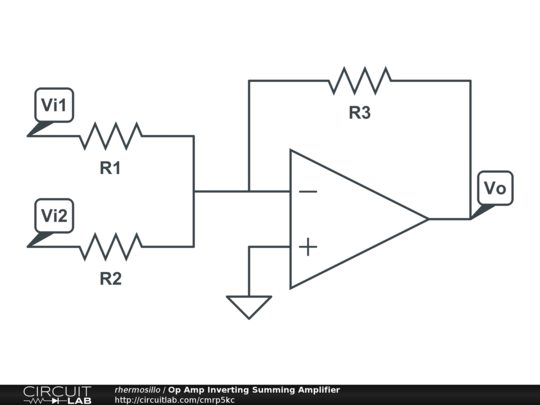
\includegraphics[width=0.70\textwidth]{schematics/invsummingamp.PNG}
\end{center}

This circuit multiplies each input voltage by a factor determined by a resistor ratio, sums these amplified voltages, and inverts the result.
It is essentially an op amp inverting amplifier with multiple inputs.
It is often used as an audio mixer, where multiple voltage signals must be combined into one (for example, voltage signals from multiple microphones which must be combined into one signal for recording).
The transfer function can be found by superposition of the inputs and, for the two input case, is

\textcolor{red}{
\begin{equation}
\vout = -\left(\frac{R_3}{R_1}\vin[1] + \frac{R_3}{R_2}\vin[2]\right)
\label{eq:invertingsummingamplifier}
\end{equation}
}

%To minimize the error due to the op amp's input bias currents $R_{5}$ should equal $R_{1}||R_{2}||R_{3}||R_{4}$.

\section{Non-inverting summing amplifier}
\begin{center}
	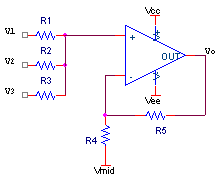
\includegraphics{schematics/summingamp.PNG}
\end{center}
The non-inverting summing amplifier is similar to the op amp non-inverting amplifier, except that it has multiple inputs. To analyze it, note that the inverting input voltage $v_{-}$ is

\begin{equation}
v_{-} = \frac{R_4}{R_4 + R_5}\vout
\end{equation}

(assume for simplicity that $V\sub{REF} = \SI{0}{\V}$) since $R_4$ and $R_5$ form a voltage divider.
This is also the voltage at the non-inverting input and \ac{kcl} can be used on the currents through the input resistors.
This gives the transfer function:

\textcolor{red}{
\begin{equation}
\vout = \frac{R_4 + R_5}{R_4\left(\frac{1}{R_1} + \frac{1}{R_2} + \frac{1}{R_3}\right)}\left(\frac{v_1}{R_1} + \frac{v_2}{R_2} + \frac{v_3}{R_3}\right)
\label{eq:summingamp}
\end{equation}
}

Determining the correct resistor values to use in order to achieve the desired gain for each input (and finding the standard resistor values that will do it) is slightly trickier than the inverting summing amplifier's case.
For audio circuits the inverting summing amplifier is easier to work with since a voltage signal that has been inverted cannot be distinguished by the human ear from the same signal that has not -- only amplitude and frequency matter in this case, not phase.
Other applications may also allow for an inversion, but if not the non-inverting summing amplifier works well.

\section{Difference Amplifiers}

\subsection{Basic difference amplifier}
\begin{center}
	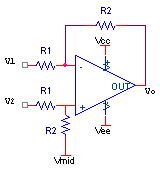
\includegraphics{schematics/differenceamp.PNG}
\end{center}
In this configuration each of the two inputs is connected to one of the op amp's inputs through a resistor ($R_1$).
Two additional resistors are used:
a feedback resistor from the output to the inverting input of the op amp, and another resistor of equal value from the non-inverting input of the op amp to the common mode voltage (usually $V\sub{CC}/2$ for a single supply system and GND for a dual supply system).
Using the fact that an ideal op amp's inputs are at equal voltages and \ac{kcl} on both the inverting and non-inverting inputs, the transfer function is

\textcolor{red}{
\begin{equation}
\vout = \frac{R_2}{R_1}(v_2 - v_1)
\label{eq:differenceamp}
\end{equation}
}

\subsection{High common-mode range difference amplifier}
\begin{center}
	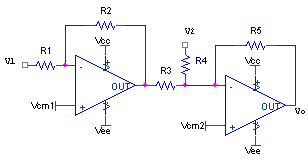
\includegraphics{schematics/highcmdifferenceamplifier.PNG}
\end{center}
This improved difference amplifier allows for a higher common-mode range because the resistors in series with the signal inputs $v_1$ and $v_2$ ($R_1$ and $R_4$, respectively) limit the currents into the op amps' inputs, increasing the voltage range within the op amp's drive capability. \autocite[418]{op-amps-for-everyone}

The transfer function can be derived easily using superposition and the above transfer functions for inverting and non-inverting op amp amplifiers to determine \vout in terms of all four inputs ($v_1$, $v_2$, $V\sub{CM1}$, and $V\sub{CM2}$).
For $v_1$,

\begin{equation}
\vout = \frac{R_2}{R_1}\frac{R_5}{R_3}v_1, v_2 = V\sub{CM1} = V\sub{CM2} = 0
\end{equation}

(the output of the first op amp is $-(R_2/R_1)v_1$, which is then amplified by $-R_5/R_3$).
For $v_2$,

\begin{equation}
\vout = -\frac{R_5}{R_4}v_2, v_1 = V\sub{CM1} = V\sub{CM2} = 0
\end{equation}

For $V\sub{CM1}$,

\begin{equation}
\vout = -\left(1+\frac{R_2}{R_1}\right)\frac{R_5}{R_3}V\sub{CM1}, v_{1} = v_{2} = V\sub{CM2} = 0
\end{equation}

For $V\sub{CM2}$,

\begin{equation}
\vout = \left(1+\frac{R_5}{R_3 \parallel R_4}\right)V\sub{CM2} = \left(1+\frac{(R_3+R_4)R_5}{R_3R_4}\right)V\sub{CM2}, v_1 = v_2 = V\sub{CM2} = 0
\end{equation}

Putting it all together,

\textcolor{red}{
\begin{equation}
\vout = \frac{R_2}{R_1}\frac{R_5}{R_3}v_1 - \frac{R_5}{R_4}v_2 - \left(1+\frac{R_2}{R_1}\right)\frac{R_5}{R_3}V\sub{CM1} + \left(1+\frac{(R_3+R_4)R_5}{R_3R_4}\right)V\sub{CM2}
\label{eq:highcmdifferenceamplifier}
\end{equation}
}

If all the resistors are equal, the transfer function simplifies to

\textcolor{red}{
\begin{equation}
\vout = v_1-v_2-2V\sub{CM1}+3V\sub{CM2}
\label{eq:highcmdifferenceamplifier_simple}
\end{equation}
}

% TODO
%\section{Op Amp Current Doubler}
% see p. 17 of the OPA454 datasheet. Slave amplifier is essentially a buffer in parallel with an op amp circuit (in any configuration)
% Also add somewhere that you can add a class B push-pull output stage to increase the current output of the op amp (see also p. 17 of the OPA454 datasheet). Put in a separate composite amplifier chapter?
